%==================================================================================================
\chapter{Acoplamento Fluido-Estrutura} \label{AFE}
%==================================================================================================

Para se descrever o problema acoplado, denota-se $\Omega_F$ o domínio do fluido, $\Omega_S$ o domínio da estrutura, $\Omega_\mathrm{IFE}=\Omega_F\cup\Omega_S$ o domínio do problema e $\Gamma_\mathrm{IFE}=\Omega_F\cap\Omega_S$ a interface de IFE, conforme ilustrado na Figura \ref{fig:DomComp}.

\begin{figure}[h!]
    \centering
    \caption{Domínio computacional do problema de IFE.}
    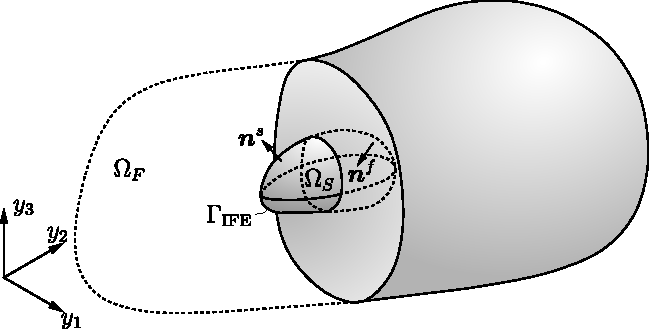
\includegraphics[width=.65\linewidth]{Figuras/Dom_Comp.pdf}
    \\Fonte: Autoria Própria (\the\year).
    \label{fig:DomComp}
\end{figure}

\citeonline{richter2017fluid} apontam três condições que devem ser satisfeitas no acoplamento: a Condição Cinemática, que diz respeito à movimentação dos domínios analisados, devendo ser compatíveis em $\Gamma_\mathrm{IFE}$, ou seja, a componente normal ao movimento deve ser igual em ambos os meios, assim como a componente tangencial em caso de condição de aderência do fluido à estrutura; a Condição Dinâmica, que aponta a continuidade das forças internas, observadas no tensor de tensões de Cauchy; e a Condição Geométrica, que exige a necessidade de ambos os domínios coincidirem em $\Gamma_\mathrm{IFE}$, não havendo sobreposições nem formação de vazios.

Numericamente, há diversas possibilidades para que essas condições sejam impostas de forma exata ou aproximada, sendo possível acoplamento monolítico ou acoplamento particionado, com o último ainda subdividido em particionado fraco e forte, como mencionado em \ref{IFE}.

Nas formulações adotadas para CFD e CSD, é comumente empregado o Método de Newton-Raphson para o cálculo das variáveis incógnitas. O mesmo pode ser aplicado quando do acoplamento direto, monolítico, entre os dois meios. Para isso a matriz tangente ($\BB{H}$) pode ser obtida por \cite{bazilevs2013computational,sanches2022metodos}:

\begin{equation}
    \BB{H}^k=\frac{\partial^2{G}}{\partial\BB{\Psi}^k\otimes\partial\DOF^k}\text{,}
\end{equation}

\noindent sendo $\script{G}$ a soma de todas as equações diferenciais do problema em sua forma fraca, $\BB{\Psi}^k$ o vetor com todos os parâmetros nodais das funções teste e $\DOF^k$ o vetor com todos os parâmetros nodais incógnitas do problema. Assim, obtém-se a correção dos valores das variáveis ($\Delta\DOF^k$) por meio da solução do sistema:

\begin{equation}
    \BB{H}^k\cdot\Delta\DOF^k=-\res^k\text{,}
\end{equation}

\noindent em que $\res^k=\partial\script{G}/\partial\BB{\Psi}^k$ é o vetor resíduo.

Expandindo a matriz em submatrizes a fim de visualizar a contribuição de cada parcela no sistema global tem-se:

\begin{equation}
    \begin{bmatrix}
        \BB{H}_{11}^k & \BB{H}_{12}^k & \BB{H}_{13}^k \\
        \BB{H}_{21}^k & \BB{H}_{22}^k & \BB{H}_{23}^k \\
        \BB{H}_{31}^k & \BB{H}_{32}^k & \BB{H}_{33}^k
    \end{bmatrix}\cdot\begin{bmatrix}
        \Delta\DOF_1^k \\\Delta\DOF_2^k\\\Delta\DOF_3^k
    \end{bmatrix}=-\begin{bmatrix}
        \res_1^k \\\res_2^k\\\res_3^k
    \end{bmatrix}\text{,}
\end{equation}

\noindent sendo os subíndices $1$, $2$ e $3$ referentes às variáveis do fluido, da estrutura e da malha, respectivamente.

Já o acoplamento particionado trata o sistema de forma a eliminar os termos cruzados da matriz tangente, resultando em blocos de sistema que podem ser resolvidos independentemente:

\begin{equation}
    \begin{bmatrix}
        \BB{H}_{11}^k & 0             & 0             \\
        0             & \BB{H}_{22}^k & 0             \\
        0             & 0             & \BB{H}_{33}^k
    \end{bmatrix}\cdot\begin{bmatrix}
        \Delta\DOF_1^k \\\Delta\DOF_2^k\\\Delta\DOF_3^k
    \end{bmatrix}=-\begin{bmatrix}
        \res_1^k \\\res_2^k\\\res_3^k
    \end{bmatrix}\text{.}
\end{equation}

Note que o método continua sendo consistente, uma vez que apenas a matriz tangente do método de Newton-Raphson foi modificada, no entanto, a convergência não é garantida.
Para aprimorar os resultados, em cada iteração $k$ do processo de Newton-Raphson, pode-se resolver sequencialmente os blocos e atualizar os valores calculados em um bloco para o cálculo do próximo, sendo obtido pelo procedimento apresentado no Algoritmo \ref{alg:acoplamentoForte}. Isso resulta em um acoplamento forte, onde, havendo convergência, a mesma resposta do problema fortemente acoplado deve ser alcançada.

\begin{algorithm}[h!]
    \caption{Processo de acoplamento particionado forte}
    \label{alg:acoplamentoForte}
    \ForEach{\textnormal{passo de tempo}}{
        Atualizar valores passados do fluido, sólido e malha;\\
        \ForEach{\textnormal{iteração $k$ de Newton-Raphson}}{
            \textbf{Resolver fluido}: $\BB{H}_{11}^k(\DOF_1^k,\DOF_2^k,\DOF_3^k)\cdot\Delta\DOF_1^k=-\res_1^k(\DOF_1^k,\DOF_2^k,\DOF_3^k)$\\
            Atualizar valores atuais do fluido: $\DOF_1^{k+1}\gets\DOF_1^k+\Delta\DOF_1^k$\\
            Atualizar forças de superfície no sólido: $\BB{t}^s=-\BB{\sigma}^f\cdot\BB{n}^f$\\
            \textbf{Resolver sólido}: $\BB{H}_{22}^k(\DOF_1^{k+1},\DOF_2^k,\DOF_3^k)\cdot\Delta\DOF_2^k=-\res_2^k(\DOF_1^{k+1},\DOF_2^k,\DOF_3^k)$\\
            Atualizar valores atuais do sólido:  $\DOF_2^{k+1}\gets\DOF_2^k+\Delta\DOF_2^k$\\
            Atualizar velocidades e acelerações do fluido em $\Gamma_\mathrm{IFE}$;\\
            Atualizar deslocamentos e acelerações na malha em $\Gamma_\mathrm{IFE}$;\\
            \textbf{Resolver malha}: $\BB{H}_{33}^k(\DOF_1^{k+1},\DOF_2^{k+1},\DOF_3^k)\cdot\Delta\DOF_3^k=-\res_3^k(\DOF_1^{k+1},\DOF_2^{k+1},\DOF_3^k)$\\
            Atualizar valores atuais da malha: $\DOF_3^{k+1}\gets\DOF_3^k+\Delta\DOF_3^k$\\
        }
    }
\end{algorithm}

Caso os blocos sejam resolvidos em processos iterativos separados, sem que haja atualização das variáveis de um problema para o outro dentro de cada processo iterativo, fazendo a atualização apenas ao final de cada passo no tempo, tem-se um modelo de acoplamento particionado fraco. Para construir um acoplamento particionado fraco, pode-se assumir que o problema do fluido depende das variáveis do sólido e da malha em um instante $t$ e das variáveis do fluido em um instante $t+1$, já o problema do sólido depende do valor das variáveis do fluido e do sólido em um tempo $t+1$ e, por fim, o problema da malha depende das variáveis do sólido e da malha em um instante $t+1$. Assim, o cálculo é realizado segundo o Algoritmo \ref{alg:PartFraco}, no qual $k_f$, $k_s$ e $k_m$ são as iterações das soluções dos problemas de fluido, estrutura e malha, respectivamente \cite{sanches2022metodos}. Ainda é observado que a movimentação da malha segue um problema linear, sendo seu resultado obtido diretamente em uma iteração.

\begin{algorithm}[h!]
    \caption{Processo de acoplamento particionado fraco}
    \label{alg:PartFraco}

    \ForEach{\textnormal{iteração $k_f$ de Newton-Raphson}}{
    Resolver o sistema: $\BB{H}_{11}((\DOF_1^{k_f})^{t+1},(\DOF_2)^t,(\DOF_3)^t)\cdot\Delta(\DOF_1^{k_f})^{t+1}=-\res_1((\DOF_1^{k_f})^{t+1},(\DOF_2)^t,(\DOF_3)^t)$\;
    Atualizar valores: $(\DOF_1^{k_f+1})^{t+1}\gets(\DOF_1^{k_f})^{t+1}+(\Delta\DOF_1^{k_f})^{t+1}$\;
    }
    Atualizar forças de superfície no sólido: $\BB{t}^s=-\BB{\sigma}^f\cdot\BB{n}^f$\\
    \ForEach{\textnormal{iteração $k_s$ de Newton-Raphson}}{
    Resolver o sistema: $\BB{H}_{22}((\DOF_1)^{t+1},(\DOF_2^{k_s})^{t+1})\cdot\Delta(\DOF_2^{k_s})^{t+1}=-\res_2((\DOF_1)^{t+1},(\DOF_2^{k_s})^t)$\;
    Atualizar valores: $(\DOF_2^{k_s+1})^{t+1}\gets(\DOF_2^{k_s})^{t+1}+(\Delta\DOF_2^{k_s})^{t+1}$\;
    }
    Atualizar velocidades e acelerações do fluido em $\Gamma_\mathrm{IFE}$;\\
    Atualizar deslocamentos e acelerações na malha em $\Gamma_\mathrm{IFE}$;\\
    \ForEach{\textnormal{iteração $k_m$ de Newton-Raphson}}{
    Resolver o sistema: $\BB{H}_{3}((\DOF_3^{k_m})^{t+1},(\DOF_2)^t)\cdot\Delta(\DOF_3^{k_s})^{t+1}=-\res_3((\DOF_3^{k_m})^{t+1},(\DOF_2)^t)$\;
    Atualizar valores: $(\DOF_3^{k_m+1})^{t+1}\gets(\DOF_3^{k_m})^{t+1}+(\Delta\DOF_3^{k_m})^{t+1}$\;
    }
\end{algorithm}

Por dispensar etapas de correção, esse método possui um custo computacional menor em relação ao particionado forte, no entanto exige a adoção de passos de tempo pequenos e fica sujeito a problemas de instabilidades como mencionado em \citeonline{Felippaetal2001}. Nota-se que esse tipo de acoplamento é mais adequado a problemas com escoamento compressível, onde um passo de tempo pequeno é necessário para se capturar a propagação de ondas de choque ao mesmo tempo em que a massa específica do fluido costuma ser muito menor que a do sólido.

Por outro lado, a convergência do processo de acoplamento particionado forte pode ficar prejudicada, especialmente à medida em que a massa específica do fluido e do sólido se aproximam, ou em problemas fortemente acoplados, onde uma pequena perturbação do fluido pode produzir grandes perturbações na estrutura e vice-versa. Como meios de garantir convergência nessa situação, mantendo o acoplamento particionado, pode-se adotar relaxações de Aitken, destinadas melhorar a convergência no método de Gauss-Seidel, na atualização das variáveis \cite{fernandes2019ale} ou aplicar um fator de escala sobre a matriz de massa do sólido (técnica \textit{Augmented $A_{22}$}) \cite{bazilevs2013computational}.

%==================================================================================================
\section{Exemplos de verificação}
%==================================================================================================

Na presente seção serão apresentados alguns exemplos para verificação do código implementado.

%==================================================================================================
\subsection{Cavidade bidimensional}
%==================================================================================================

O primeiro exemplo utilizado para verificação do código utilizando o acoplamento forte tipo bloco-iterativo trata-se de uma cavidade com fundo flexível, conforme ilustrado na Figura \ref{fig:cavity2D}. Tal exemplo caracteriza-se pelo comportamento bidimensional do escoamento, no entanto pode ser satisfatoriamente transportado para uma análise tridimensional, sendo apenas necessário impedir o movimento da estrutura na terceira dimensão, assim como travar essa componente do vetor generalizado. Esse problema foi estudado por \citeonline{gerbeau2003quasi}, considerando as seguintes propriedades da casca: massa específica $\rho_S=500$, módulo de Young $E=250$, coeficiente de Poisson $\nu=0$ e espessura $h=0,002$; e do fluido: massa específica $\rho_F=1$ e viscosidade dinâmica $\mu=0,01$. Na face superior da cavidade é imposta uma velocidade prescrita variável ao longo do tempo, sendo $u_1(t)=1-\cos{(0,4\pi t)}$, logo, tomando-se o comprimento característico o tamanho do lado da cavidade, o número de Reynolds varia entre 0 a 200.

\begin{figure}[h!]
    \centering
    \caption{Problema de cavidade com fundo flexível.}
    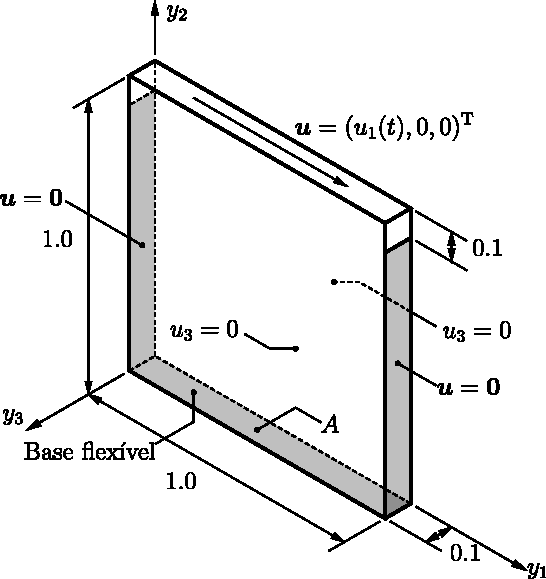
\includegraphics[width=0.5\linewidth]{Figuras/FSI-Cavity2D/FSI-Cavity2D.pdf}
    \\Fonte: Autoria Própria (\the\year).
    \label{fig:cavity2D}
\end{figure}

Para a solução do problema via MEF, considerou-se um intervalo de tempo $t\in[0,60]$ discretizado em $\Delta t=0,1$, sendo o domínio computacional referente ao fluido performado com uma malha contendo 1845 elementos, 3859 nós, o que resulta em 15436 graus de liberdade. Já o domínio computacional da casca foi realizada com uma malha contendo 60 elementos, 155 nós, resultando em 1085 graus de liberdade. A Figura \ref{fig:Cavity2D-mesh} apresenta a malha utilizada para cada um dos meios. A integração temporal foi feita considerando-se $\rho_\infty=0$, pois, como relatado por \citeonline{forster2007artificial}, integradores temporais de segunda ordem levaram a instabilidades imediatas. Os termos estabilizadores considerados foram o PSPG e SUPG.

\begin{figure}[h!]
    \centering
    \caption{Malha utilizada para o domínio:}
    \begin{subfigure}[b]{0.32\textwidth}
        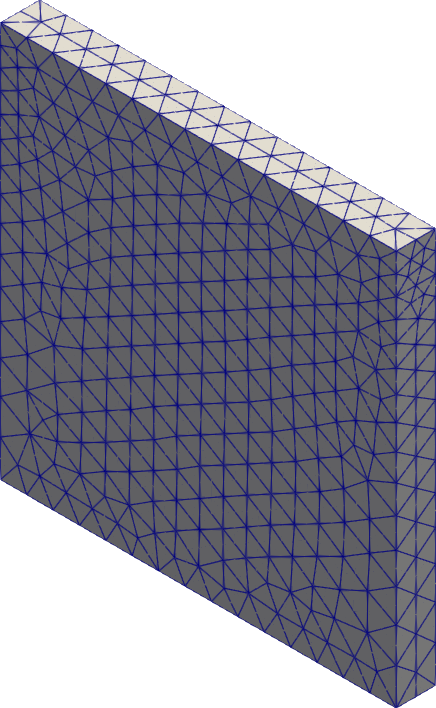
\includegraphics[width=\linewidth]{Figuras/FSI-Cavity2D/fluid-mesh.png}
        \caption{do fluido.}
    \end{subfigure}
    \begin{subfigure}[b]{0.32\textwidth}
        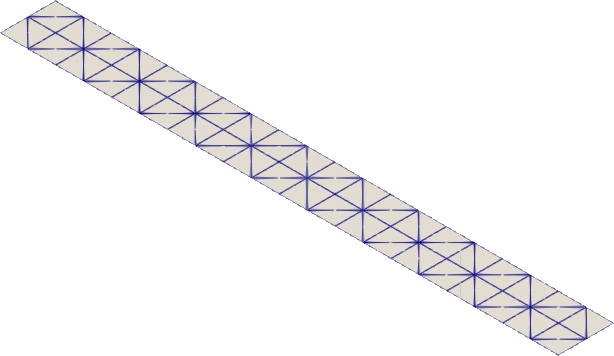
\includegraphics[width=\linewidth]{Figuras/FSI-Cavity2D/shell-mesh.png}
        \caption{da casca.}
    \end{subfigure}
    \\Fonte: Autoria Própria (\the\year).
    \label{fig:Cavity2D-mesh}
\end{figure}

Para a que fosse efetuada a transferência das condições de contorno entre os meios, utilizou-se malhas de tal forma que os nós do sólido e do fluido fossem coincidentes em $\Gamma_\mathrm{IFE}$, onde os valores das forças de superfície advindas do fluido fossem transferidas diretamente para os nós da casca, assim como as variáveis da movimentação da casca foram transferidas para o fluido e malha.

Nesse problema, observou-se instabilidades nos resultados, o que levou à necessidade de se multiplicar a parcela da matriz de massa da estrutura por uma valor de $2,0$, estabilizando, assim, os resultados.

Observou-se, portanto o deslocamento vertical do nó $A$, referente ao centro da casca, e comparou-se os resultados obtidos por \citeonline{gerbeau2003quasi} (Figura \ref{fig:cavity2D-res}).

\begin{figure}[h!]
    \centering
    \caption{Deslocamento vertical do nó $A$.}
    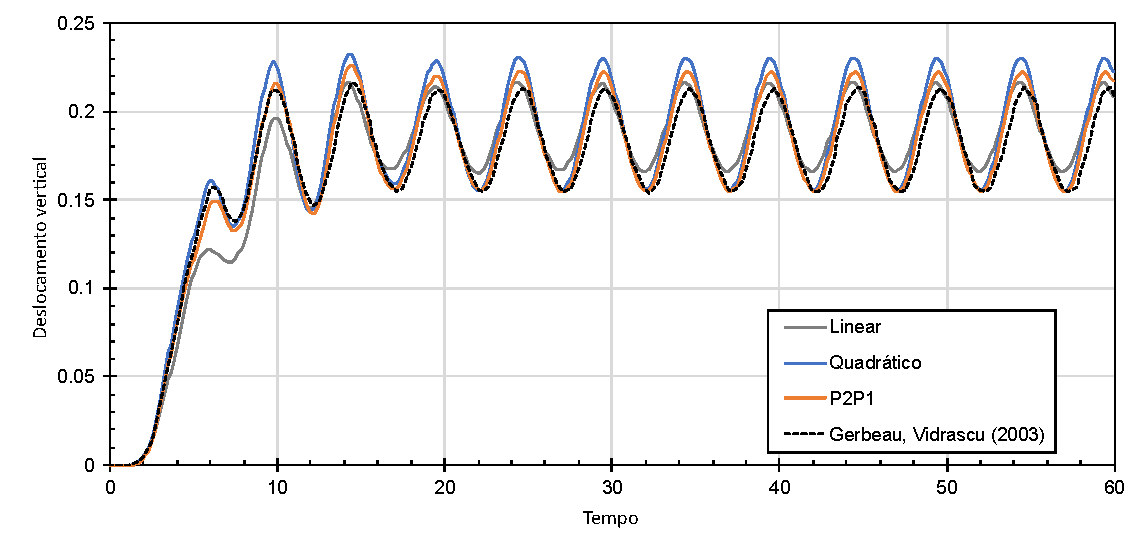
\includegraphics[width=.8\linewidth]{Figuras/FSI-Cavity2D/resultados.pdf}
    \\Fonte: Autoria Própria (\the\year).
    \label{fig:cavity2D-res}
\end{figure}

A Figura \ref{fig:cavity2D-time} apresenta o campo de pressões na cavidade, assim como as linhas de corrente, para os instantes de tempo $t=3,5$, $8,0$, $14,0$ e $21,0$, sendo próximos aos campos encontrados por \citeonline{fernandes2016interaccao}.

\begin{figure}[h!]
    \centering
    \caption{Campo de pressões e linhas de corrente na cavidade.}
    \begin{subfigure}[b]{0.3\textwidth}
        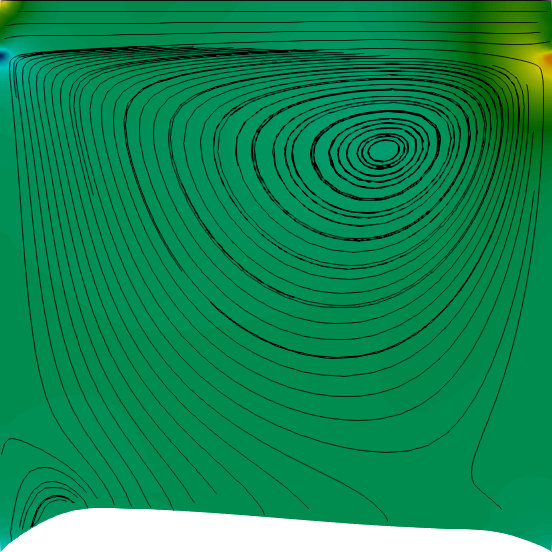
\includegraphics[width=\linewidth]{Figuras/FSI-Cavity2D/t3_5.png}
        \caption{$t=3,5$}
    \end{subfigure}
    \begin{subfigure}[b]{0.3\textwidth}
        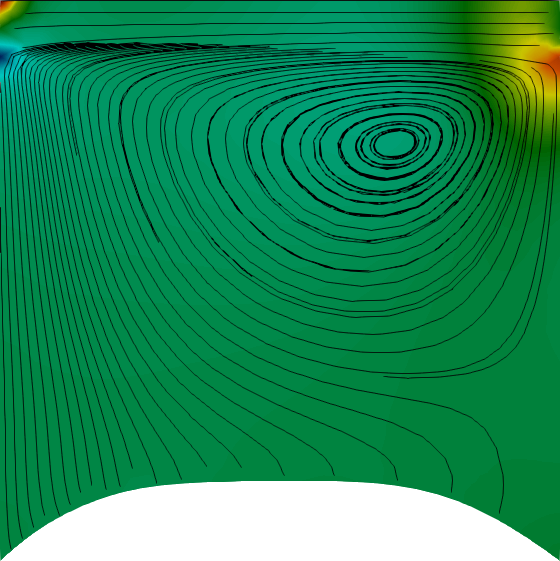
\includegraphics[width=\linewidth]{Figuras/FSI-Cavity2D/t8.png}
        \caption{$t=8,0$}
    \end{subfigure}\\
    \begin{subfigure}[b]{0.3\textwidth}
        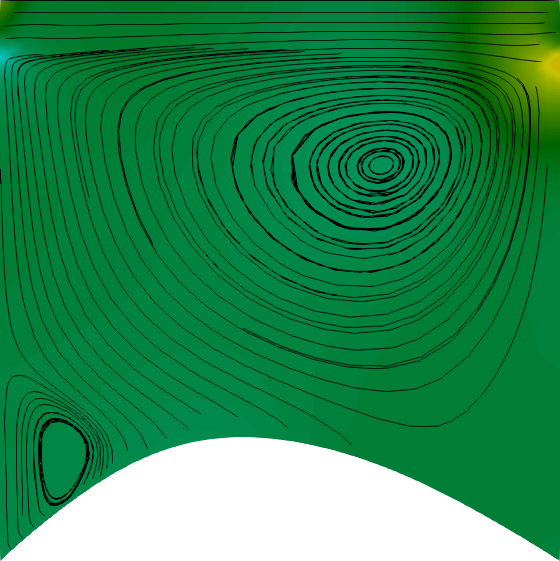
\includegraphics[width=\linewidth]{Figuras/FSI-Cavity2D/t14.png}
        \caption{$t=14,0$}
    \end{subfigure}
    \begin{subfigure}[b]{0.3\textwidth}
        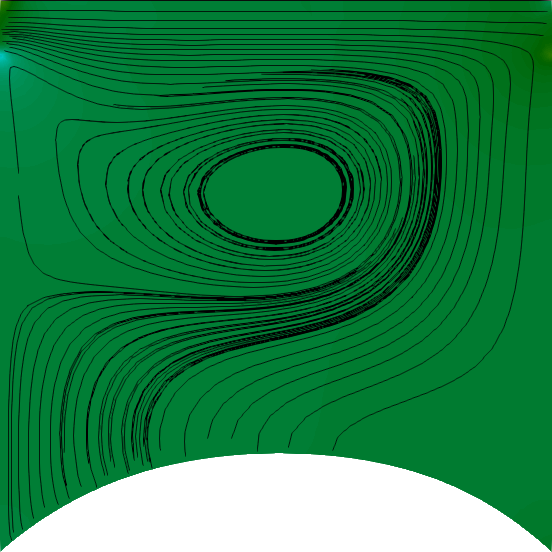
\includegraphics[width=\linewidth]{Figuras/FSI-Cavity2D/t21.png}
        \caption{$t=21,0$}
    \end{subfigure}
    \begin{subfigure}[b]{0.4\textwidth}
        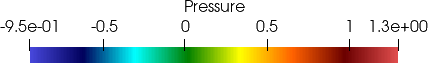
\includegraphics[width=\linewidth]{Figuras/FSI-Cavity2D/legenda.png}
    \end{subfigure}
    \\Fonte: Autoria Própria (\the\year).
    \label{fig:cavity2D-time}
\end{figure}

%==================================================================================================
\subsection{\textit{Flutter} em painel}
%==================================================================================================

Outro problema encontrado simulado trata-se de um painel engastado a um prisma quadrado rígido, como observado na Figura \ref{fig:FSI-prism}, proposto por \citeonline{wall1998fluid} e modificado por \citeonline{hubner2004monolithic}. Tal exemplo apresenta certa complexidade, uma vez que o desprendimento de vórtices ocasionado pelo escoamento em torno do prisma gera um campo de pressões de tal forma a induzir grandes deslocamentos na estrutura. O problema consiste em um painel de comprimento $L=4$ cm e espessura $h_0=0,06$ cm engastado em um bloco de dimensões $1\times 1$ cm². O painel possui módulo de Young $E=2,0\times10^6$ g/(cm$\cdot$s²), coeficiente de Poissin $\nu=0$ e massa específica $\rho_S=2,0$ g/cm³. O fluido que envolve a estrutura possui massa específica $\rho_f=1,18\times10^{-3}$ g/cm³ e viscosidade dinâmica $\mu=1,82\times10^{-4}$ g/(cm$\cdot$s), modelado em um domínio $\Omega=[0,21]\times[0,12]$ cm², com uma velocidade de entrada constante $u_\infty=31,5$ cm/s na direção 1, resultando em um número de Reynolds, considerando o comprimento característico como o lado do bloco, de $\Rey=204$. Esse problema é conhecido pelo comportamento bidimensional das variáveis envolvidas, no entanto a simulação foi realizada considerando um problema tridimensional, assim foi considerada uma espessura $e=0,1$ cm para o domínio computacional, assim como imposição de deslocamento nulo do painel na direção da espessura e do travamento dessa componente no vetor generalizado, enquanto no fluido foi considerada uma condição de não penetração nas faces frontal e traseira do domínio.

\begin{figure}[h!]
    \centering
    \caption{Problema de \textit{flutter} em painel.}
    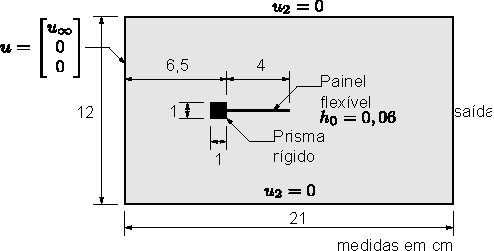
\includegraphics[width=.75\linewidth]{Figuras/FSI-prism/FSI-prism.pdf}
    \\Fonte: Autoria Própria (\the\year).
    \label{fig:FSI-prism}
\end{figure}

Segundo \citeonline{WARBURTON1976109}, o qual considera uma teoria clássica da dinâmica das estruturas, tem-se que os três primeiros modos de vibração de uma viga engastada com essas dimensões são $f_1=0,606$ Hz, $f_2=3,796$ Hz e $f_3=10,630$ Hz. Já a frequência de desprendimento de vórtices pode ser obtida ao manter toda a estrutura rígida, que segundo \citeonline{hubner2004monolithic}, resulta em $f_v=3,7$ Hz, o que se aproxima do segundo modo de vibração da estrutura, levando, portanto, à dominância desse modo.

O domínio computacional do fluido foi discretizado em 3423 elementos e 7088 nós, resultando em 28352 graus de liberdade. Já o domínio computacional da casca foi discretizado em 54 elementos e 165 nós, resultando em 1155 graus de liberdade. A Figura \ref{fig:meshPanel} apresenta as malhas utilizadas em ambos os domínios. O intervalo de tempo analisado foi $t\in[0,16]$, discretizado em passos de tempo $\Delta t=5\times10^{-3}$. O esquema de integração temporal foi dado considerando um raio espectral $\rho_\infty=0$ e os termos estabilizadores adotados foram somente o PSPG e SUPG.

\begin{figure}[h!]
    \centering
    \caption{Malha utilizada para os domínios da simulação de painel.}
    \begin{subfigure}[b]{\textwidth}
        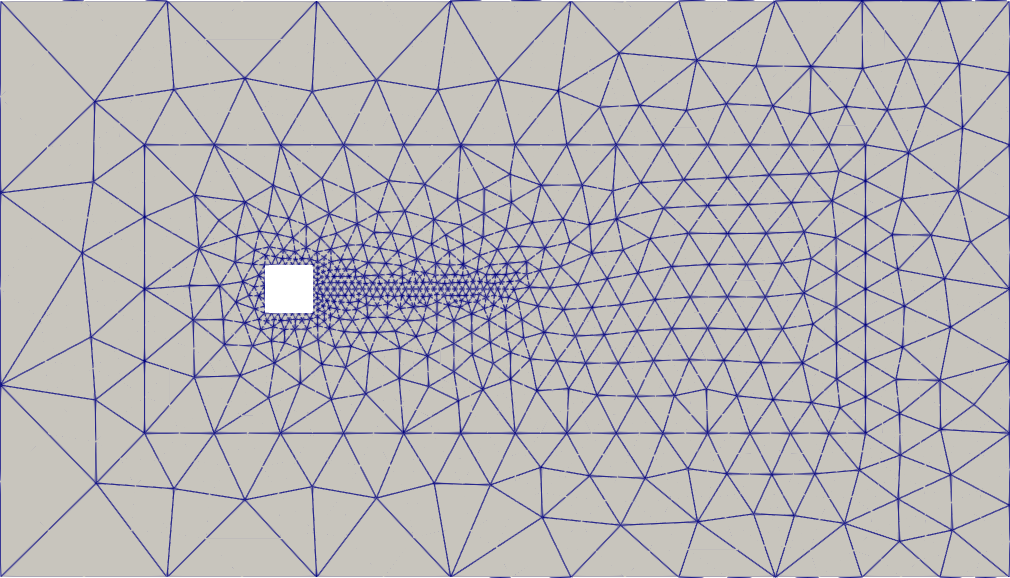
\includegraphics[width=\linewidth]{Figuras/FSI-prism/meshFluid.png}
        \caption{Malha do fluido.}
    \end{subfigure}
    \begin{subfigure}[b]{\textwidth}
        
\includegraphics[width=\linewidth]{Figuras/FSI-prism/meshSolid.png}
        \caption{Malha da casca.}
    \end{subfigure}
    \\Fonte: Autoria Própria (\the\year).
    \label{fig:meshPanel}
\end{figure}

Pelo fato do problema apresentar grandes deslocamentos, principalmente na extremidade do painel, foi alterado o fator de rigidez da equação \ref{eq:movStiff} para o valor:

\begin{equation}
    \eta^e=\frac{V_\mathrm{máx}^2-V_\mathrm{mín}^2}{2(V^e)^2}\text{,}
\end{equation}

\noindent o que aumenta consideravelmente a rigidez dos elementos menores, mantendo sua forma, enquanto os elementos maiores absorvem mais os deslocamentos da malha.

O gráfico apresentado na Figura \ref{fig:prismRes} indica o deslocamento vertical da extremidade do painel ao longo do tempo em comparação com a envoltória de deslocamentos obtido por \citeonline{hubner2004monolithic}.

\begin{figure}[h!]
    \centering
    \caption{Deslocamento vertical na extremidade do painel ao longo do tempo.}
    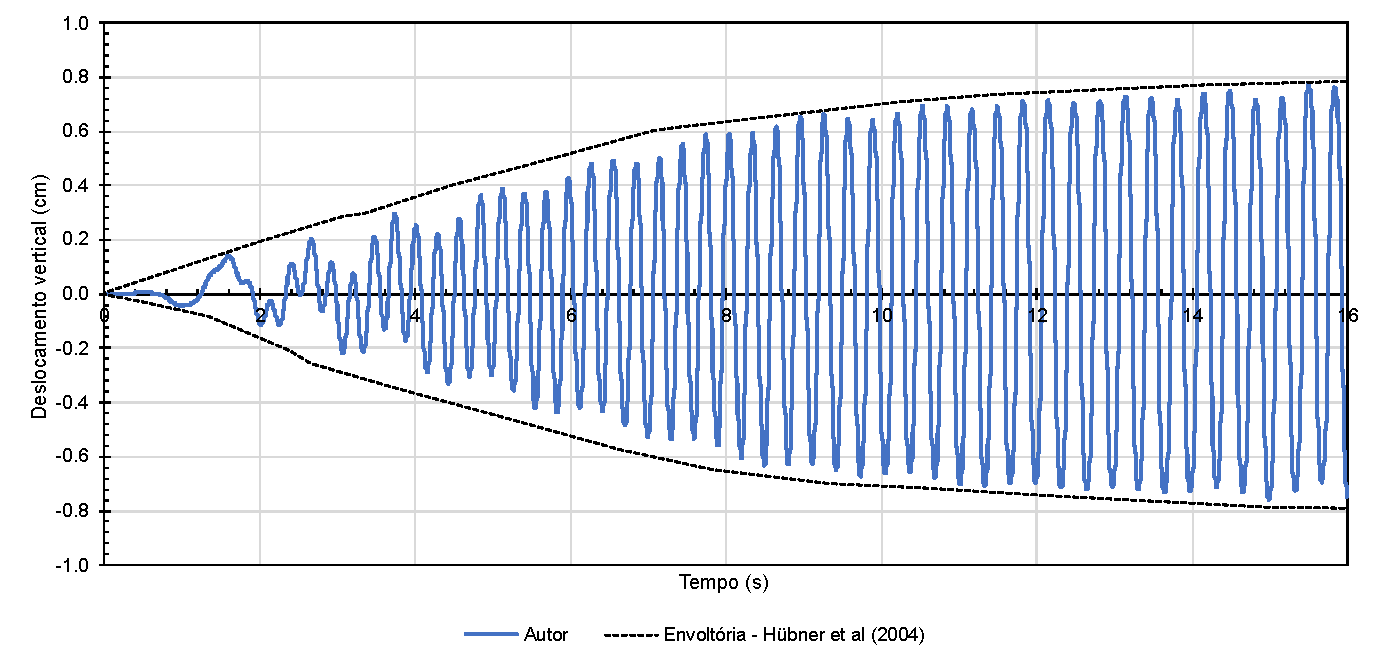
\includegraphics[width=\linewidth]{Figuras/FSI-prism/resultados.pdf}
    \\Fonte: Autoria Própria (\the\year).
    \label{fig:prismRes}
\end{figure}

Assim, observa-se que a estrutura vibra com uma frequência de 2,941 Hz, o que se aproxima do segundo modo de vibração, como esperado. Também se aproxima dos resultados de \citeonline{hubner2004monolithic}, os quais determinaram um valor de 3,1 Hz em seus resultados. Já com relação à amplitude do deslocamento, esta esteve dentro das envoltórias da referência em todo o intervalo de análise, chegando próximo à amplitude máxima encontrada pelos autores, de 0,8 cm.

Já os campos de velocidades, pressões e a configuração da malha são apresentadas em função de um período $T$ da oscilação. As Figuras \ref{fig:prismVel}, \ref{fig:prismPres} e \ref{fig:prismMesh} apresentam visualmente os campos de velocidades, pressões e a configuração da malha para frações $T/6$ do período, respectivamente. Em todos os casos, houve uma boa concordância com os campos obtidos por \citeonline{fernandes2020tecnica}.

\begin{figure}[h!]
    \centering
    \caption{Campo de magnitude de velocidades obtidos no problema de \textit{Flutter} em painel.}
    \begin{subfigure}[b]{0.49\textwidth}
        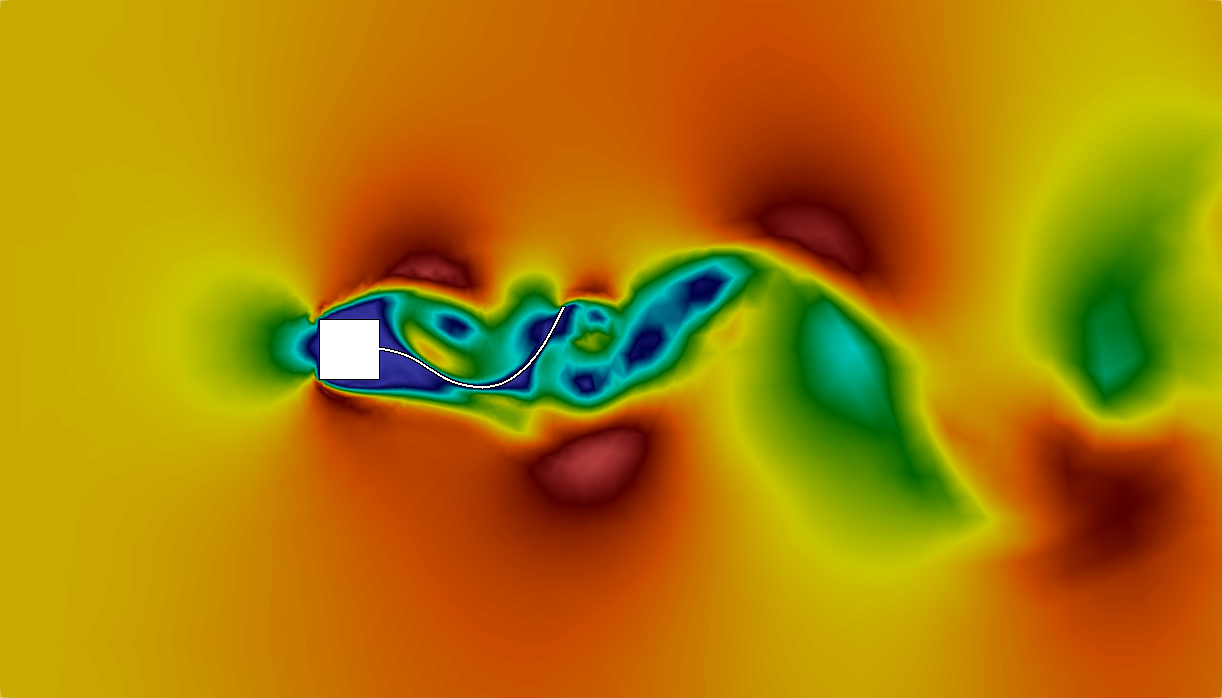
\includegraphics[width=\linewidth]{Figuras/FSI-prism/vT1.png}
        \caption{$t=nT$}
    \end{subfigure}
    \begin{subfigure}[b]{0.49\textwidth}
        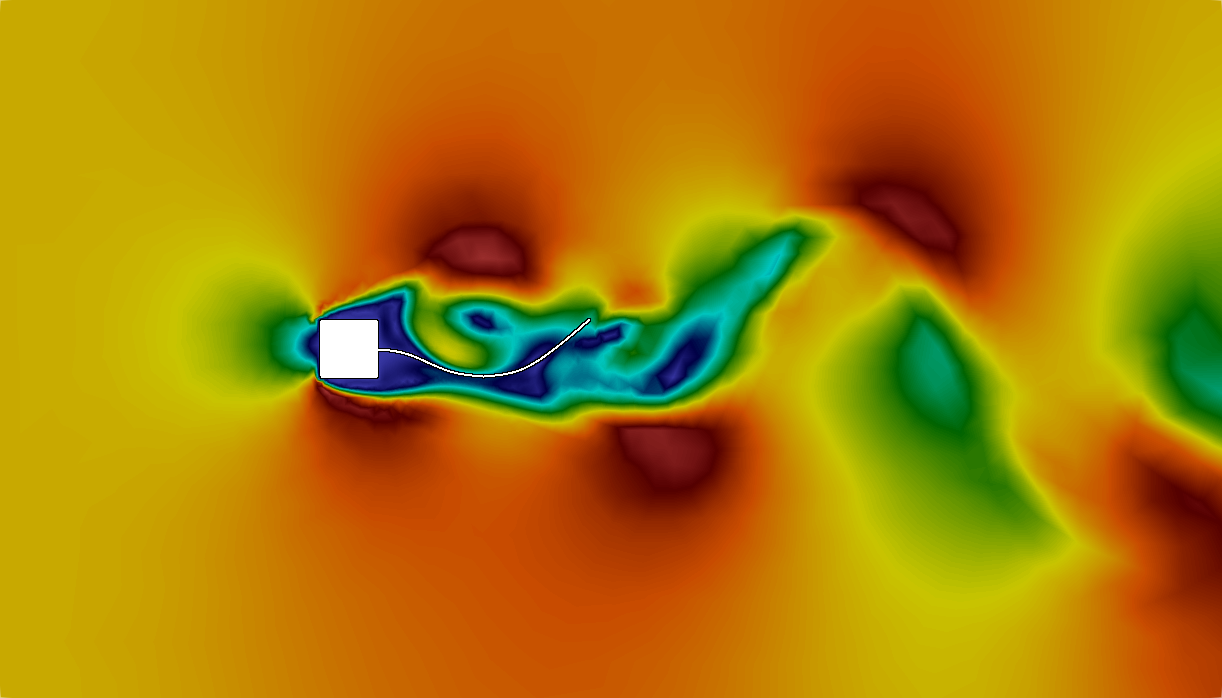
\includegraphics[width=\linewidth]{Figuras/FSI-prism/vT2.png}
        \caption{$t=nT+T/6$}
    \end{subfigure}
    \begin{subfigure}[b]{0.49\textwidth}
        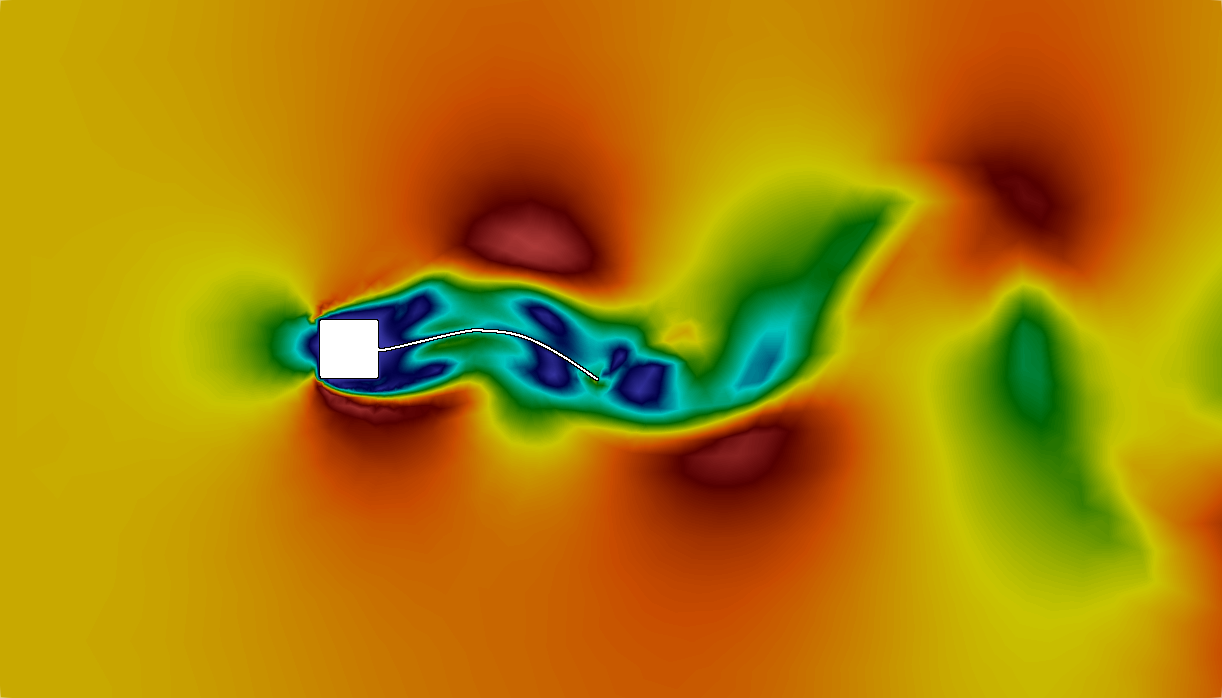
\includegraphics[width=\linewidth]{Figuras/FSI-prism/vT3.png}
        \caption{$t=nT+2T/6$}
    \end{subfigure}
    \begin{subfigure}[b]{0.49\textwidth}
        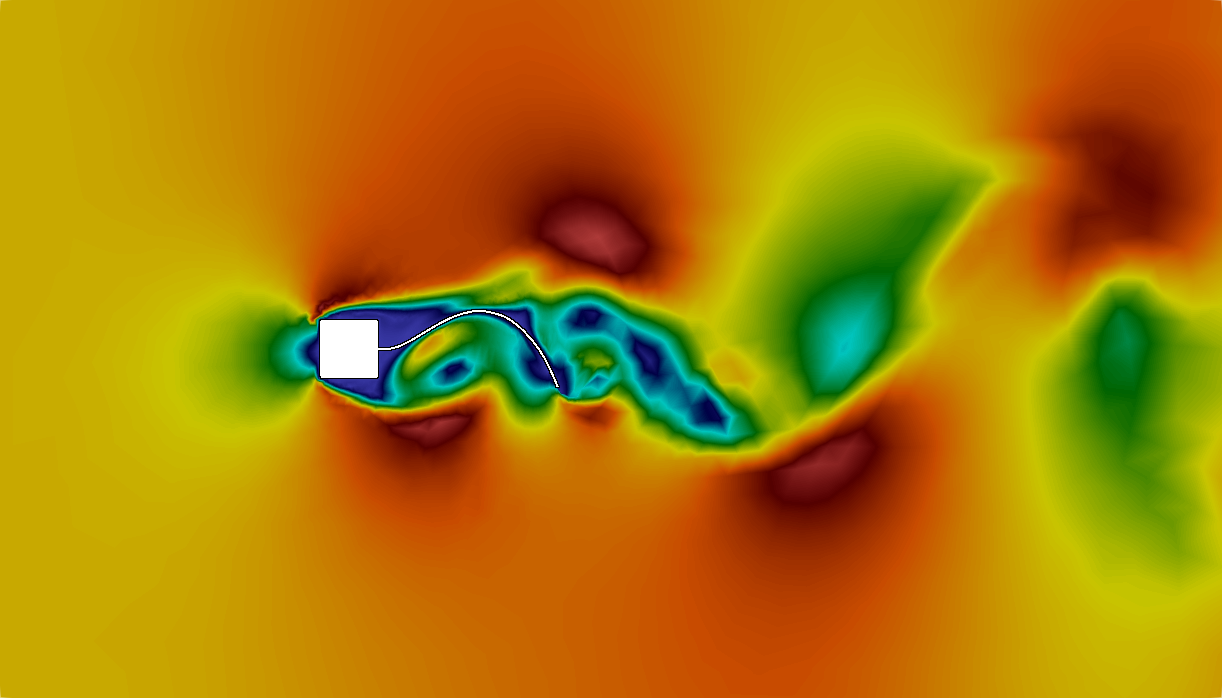
\includegraphics[width=\linewidth]{Figuras/FSI-prism/vT4.png}
        \caption{$t=nT+3T/6$}
    \end{subfigure}
    \begin{subfigure}[b]{0.49\textwidth}
        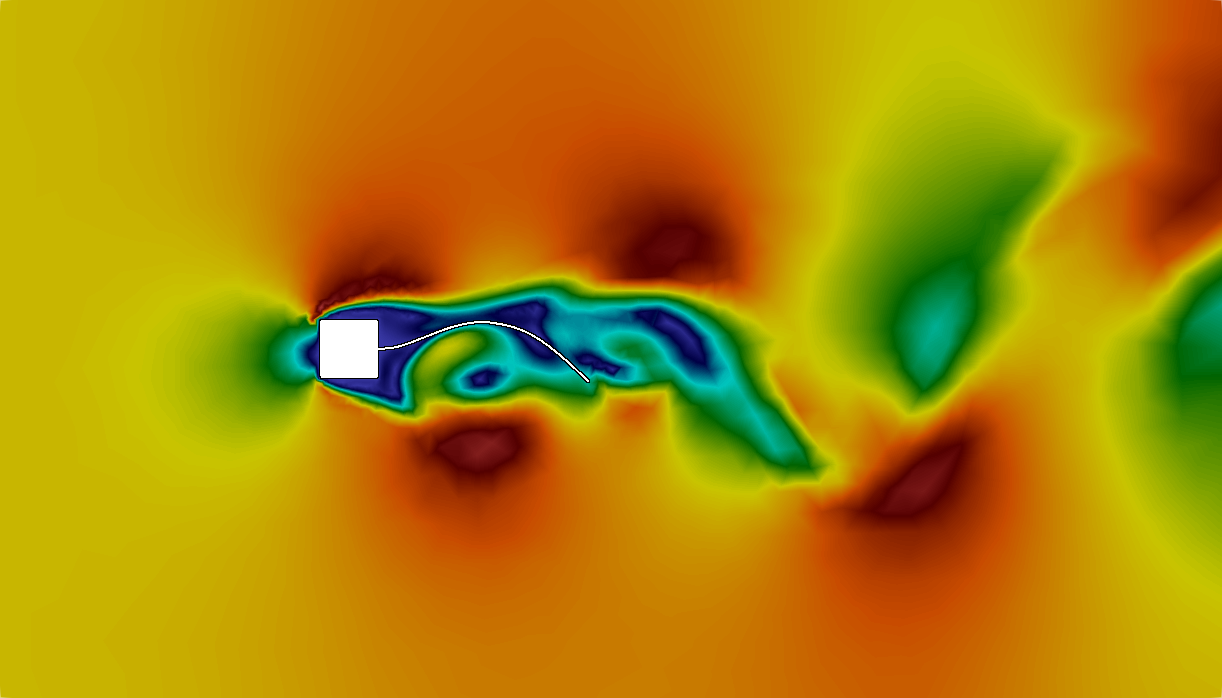
\includegraphics[width=\linewidth]{Figuras/FSI-prism/vT5.png}
        \caption{$t=nT+4T/6$}
    \end{subfigure}
    \begin{subfigure}[b]{0.49\textwidth}
        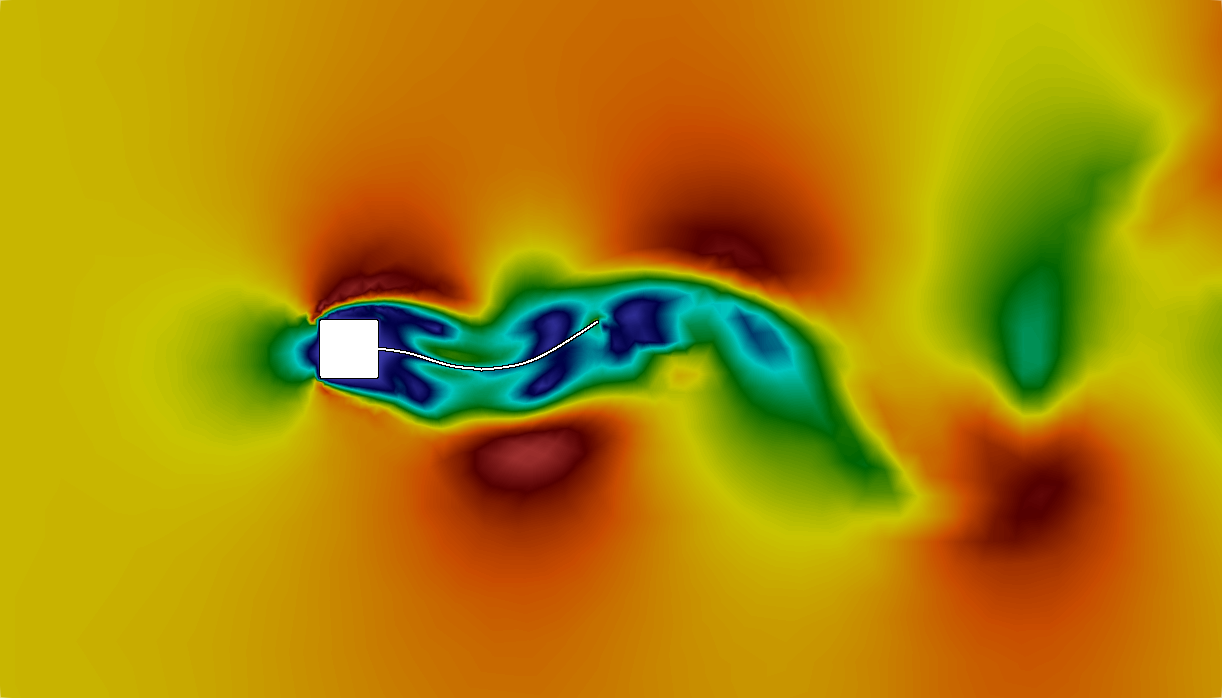
\includegraphics[width=\linewidth]{Figuras/FSI-prism/vT6.png}
        \caption{$t=nT+5T/6$}
    \end{subfigure}
    \begin{subfigure}[b]{0.49\textwidth}
        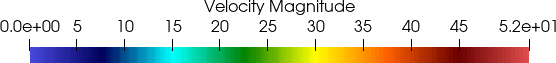
\includegraphics[width=\linewidth]{Figuras/FSI-prism/legendav.png}
    \end{subfigure}
    \\Fonte: Autoria Própria (\the\year).
    \label{fig:prismVel}
\end{figure}

\begin{figure}[h!]
    \centering
    \caption{Campo de pressões obtidos no problema de \textit{Flutter} em painel.}
    \begin{subfigure}[b]{0.49\textwidth}
        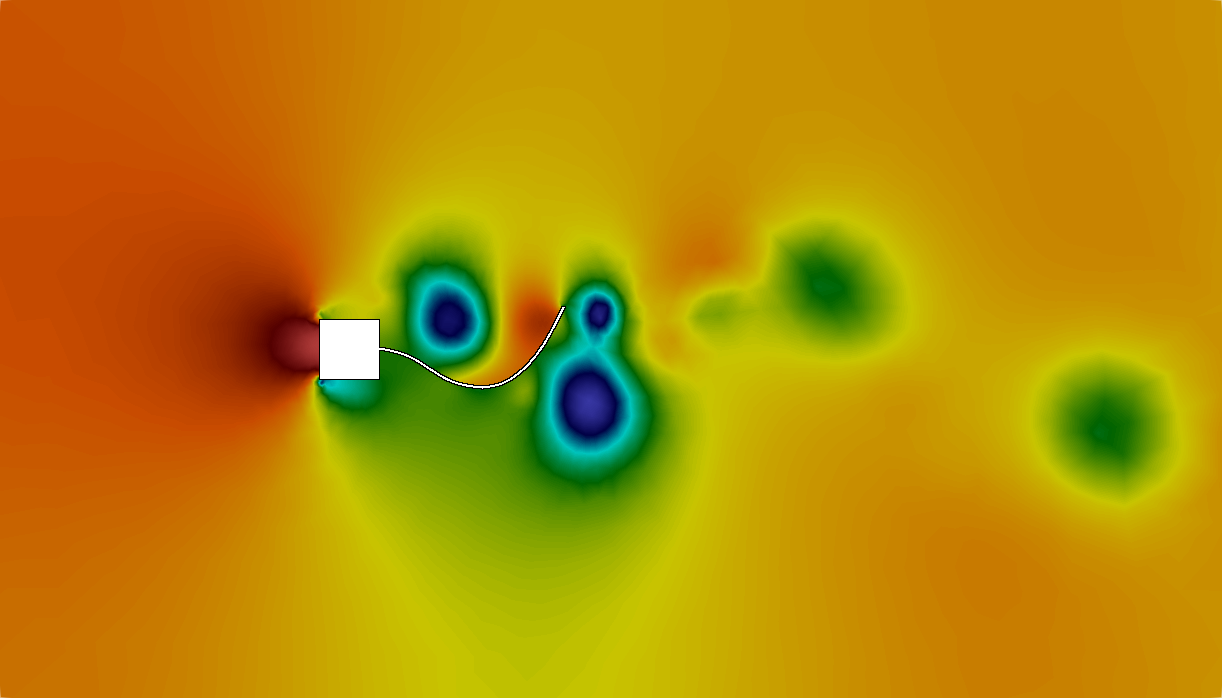
\includegraphics[width=\linewidth]{Figuras/FSI-prism/pT1.png}
        \caption{$t=nT$}
    \end{subfigure}
    \begin{subfigure}[b]{0.49\textwidth}
        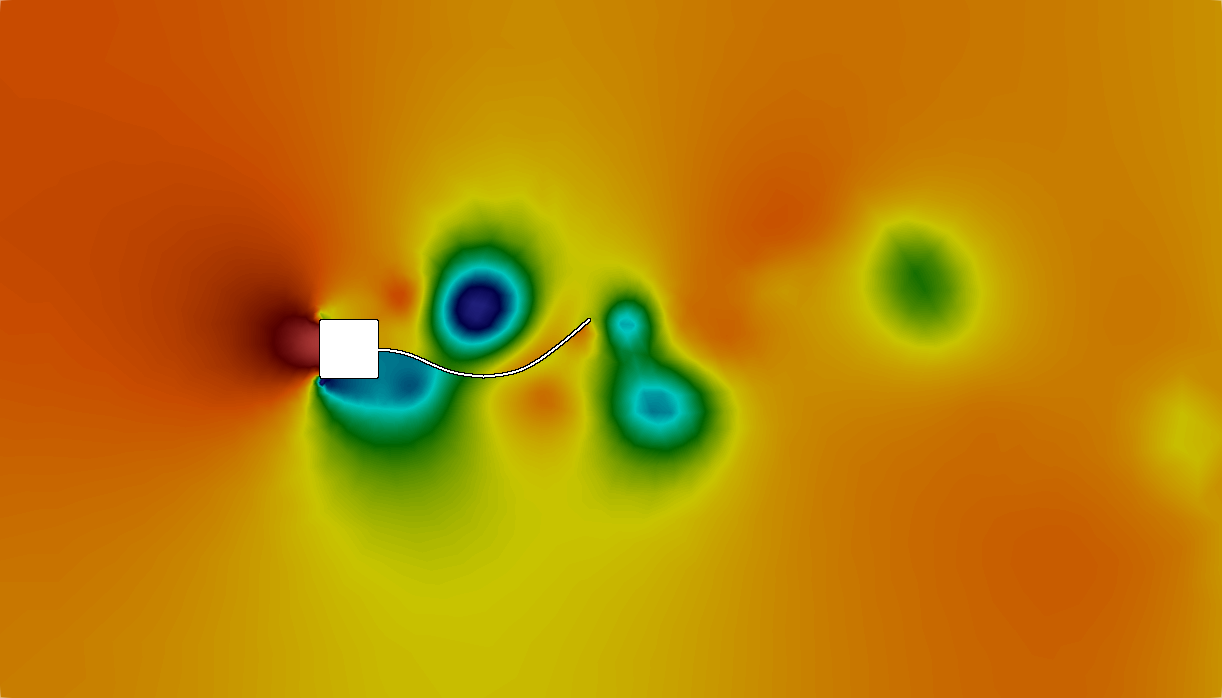
\includegraphics[width=\linewidth]{Figuras/FSI-prism/pT2.png}
        \caption{$t=nT+T/6$}
    \end{subfigure}
    \begin{subfigure}[b]{0.49\textwidth}
        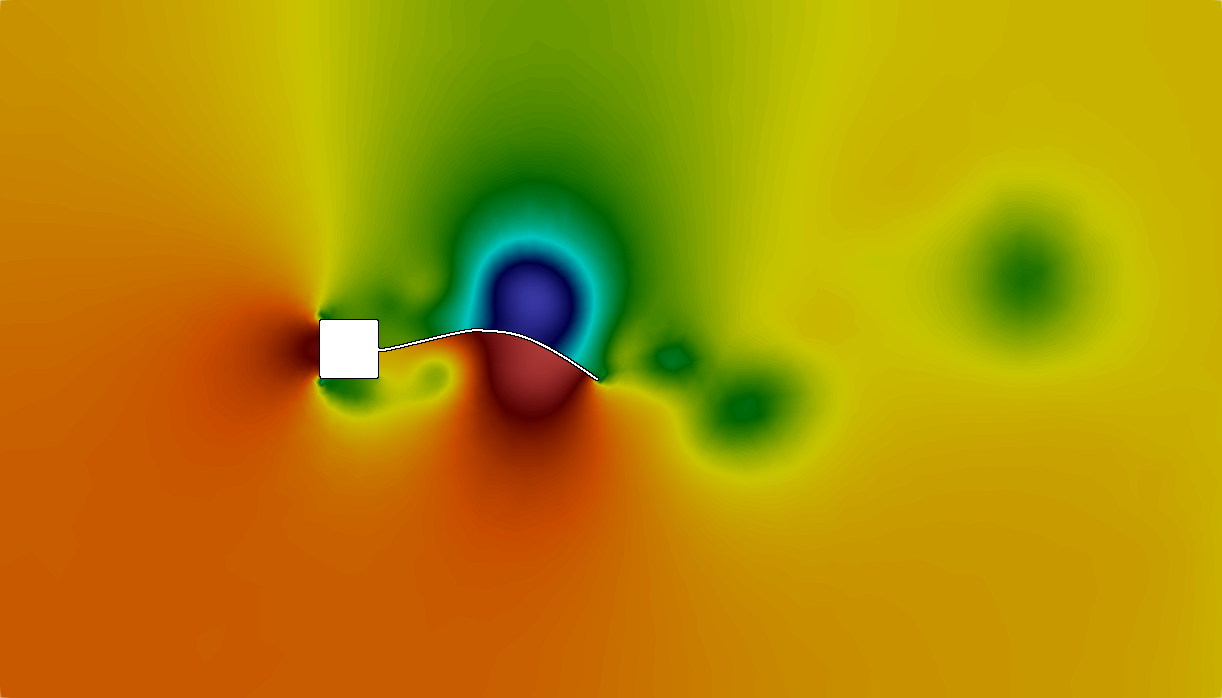
\includegraphics[width=\linewidth]{Figuras/FSI-prism/pT3.png}
        \caption{$t=nT+2T/6$}
    \end{subfigure}
    \begin{subfigure}[b]{0.49\textwidth}
        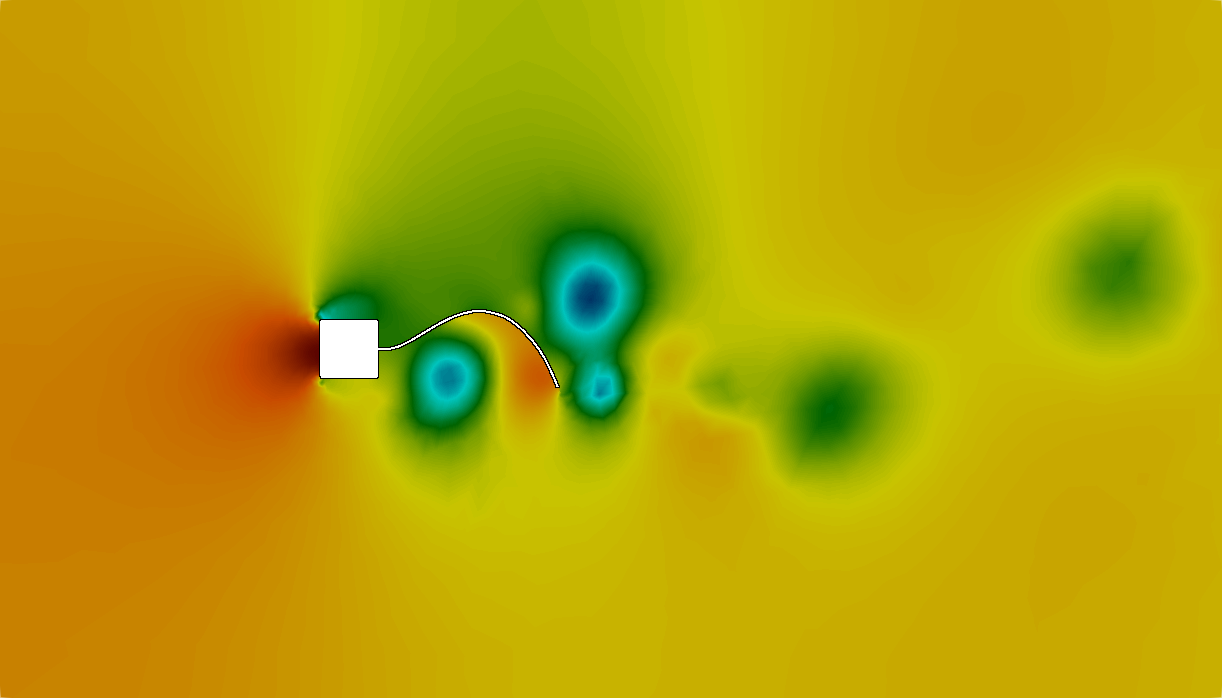
\includegraphics[width=\linewidth]{Figuras/FSI-prism/pT4.png}
        \caption{$t=nT+3T/6$}
    \end{subfigure}
    \begin{subfigure}[b]{0.49\textwidth}
        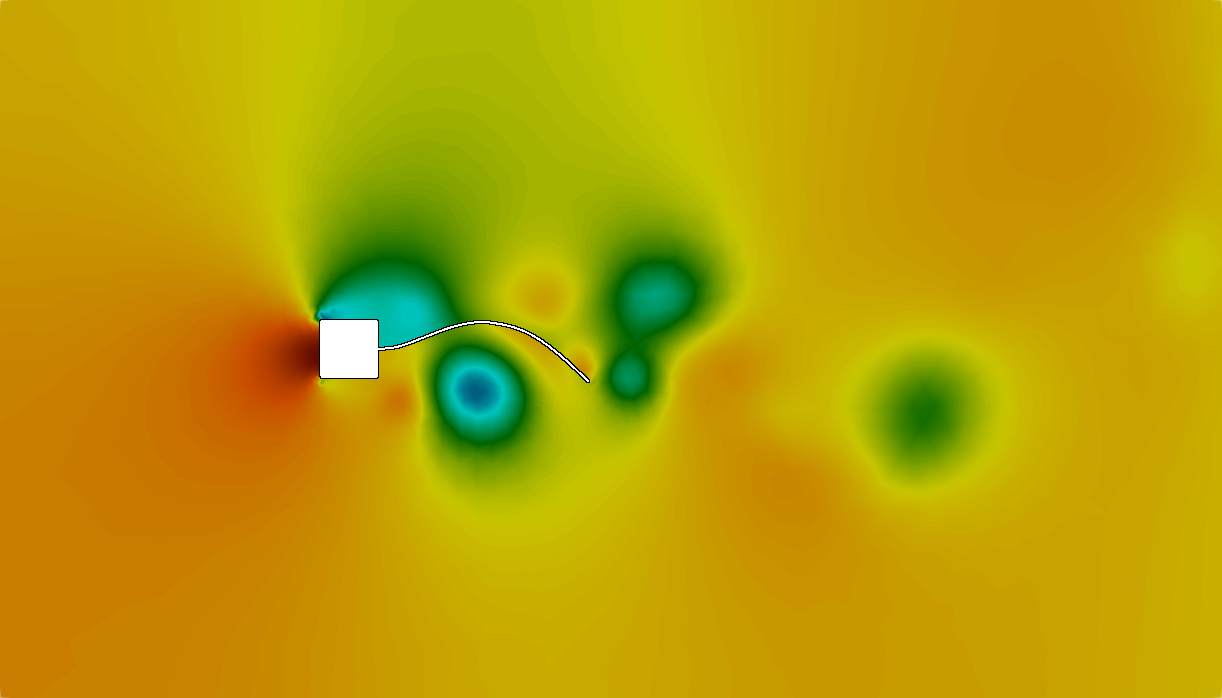
\includegraphics[width=\linewidth]{Figuras/FSI-prism/pT5.png}
        \caption{$t=nT+4T/6$}
    \end{subfigure}
    \begin{subfigure}[b]{0.49\textwidth}
        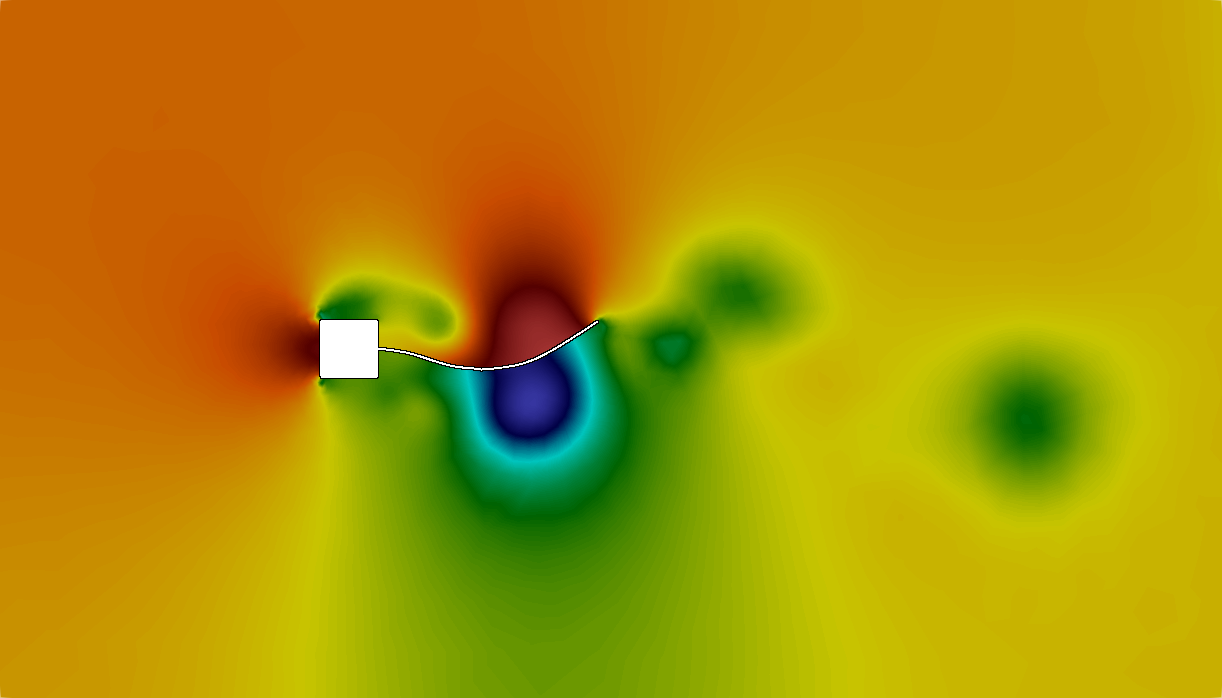
\includegraphics[width=\linewidth]{Figuras/FSI-prism/pT6.png}
        \caption{$t=nT+5T/6$}
    \end{subfigure}
    \begin{subfigure}[b]{0.49\textwidth}
        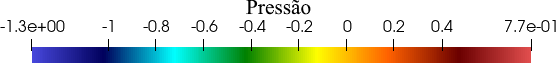
\includegraphics[width=\linewidth]{Figuras/FSI-prism/legendap.png}
    \end{subfigure}
    \\Fonte: Autoria Própria (\the\year).
    \label{fig:prismPres}
\end{figure}

\begin{figure}[h!]
    \centering
    \caption{Configurações da malha obtidas no problema.}
    \begin{subfigure}[b]{0.49\textwidth}
        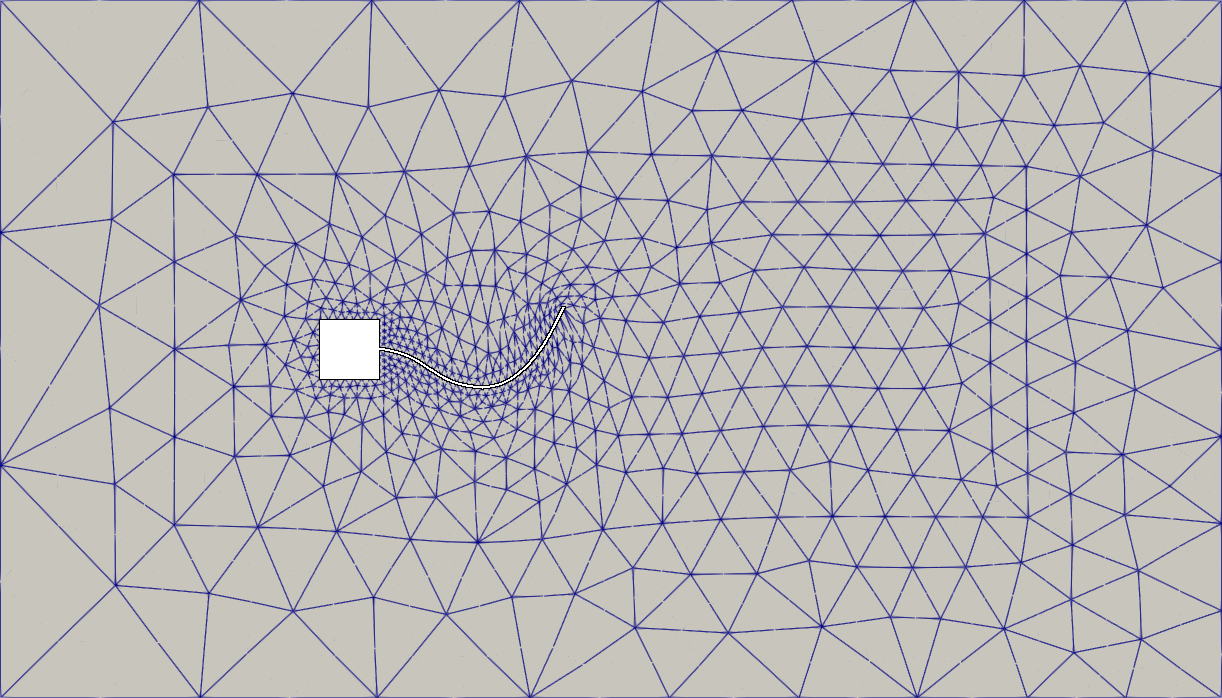
\includegraphics[width=\linewidth]{Figuras/FSI-prism/mT1.png}
        \caption{$t=nT$}
    \end{subfigure}
    \begin{subfigure}[b]{0.49\textwidth}
        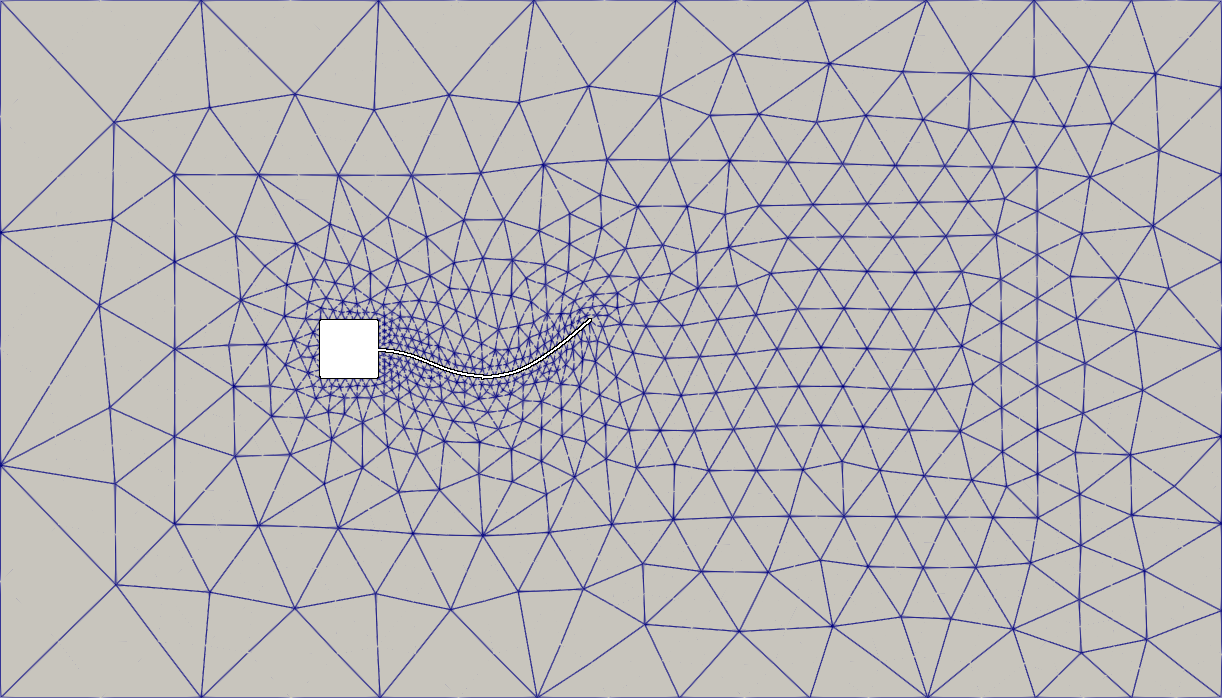
\includegraphics[width=\linewidth]{Figuras/FSI-prism/mT2.png}
        \caption{$t=nT+T/6$}
    \end{subfigure}
    \begin{subfigure}[b]{0.49\textwidth}
        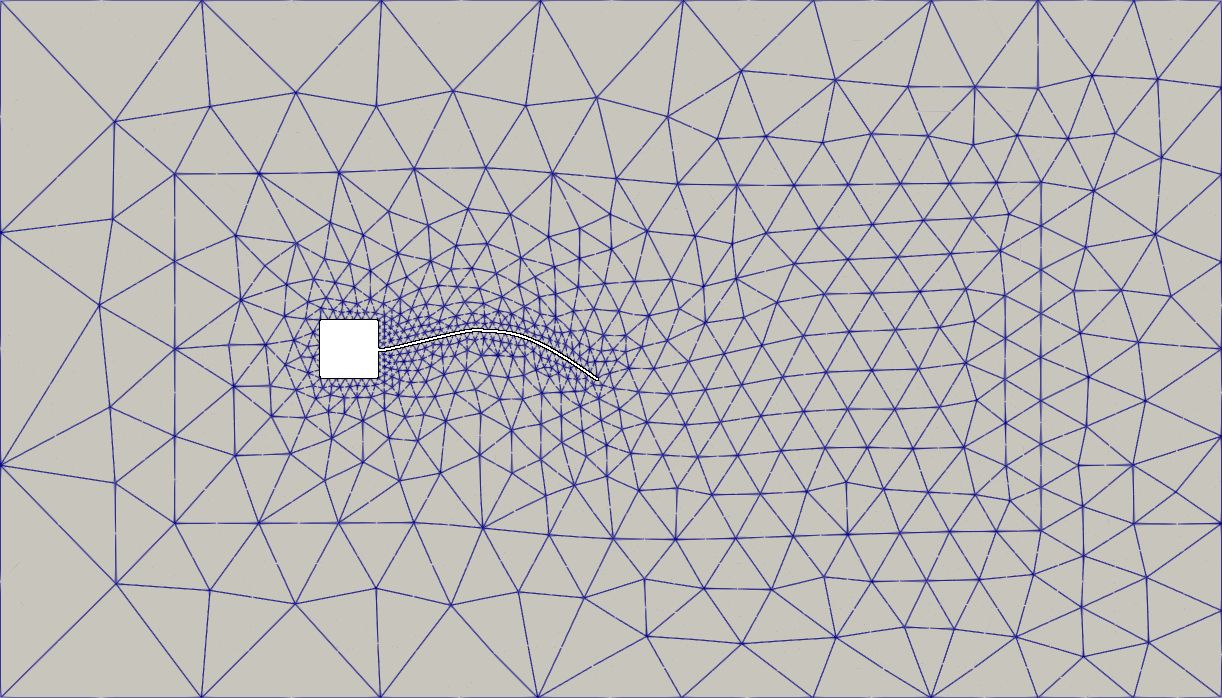
\includegraphics[width=\linewidth]{Figuras/FSI-prism/mT3.png}
        \caption{$t=nT+2T/6$}
    \end{subfigure}
    \begin{subfigure}[b]{0.49\textwidth}
        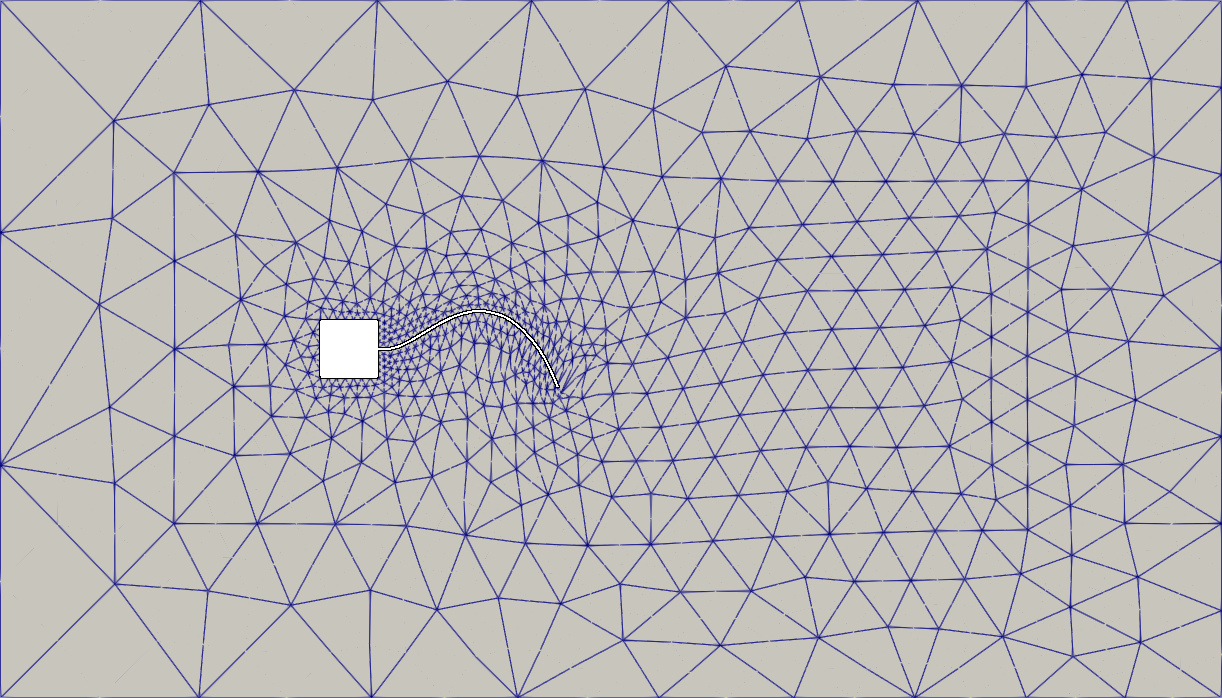
\includegraphics[width=\linewidth]{Figuras/FSI-prism/mT4.png}
        \caption{$t=nT+3T/6$}
    \end{subfigure}
    \begin{subfigure}[b]{0.49\textwidth}
        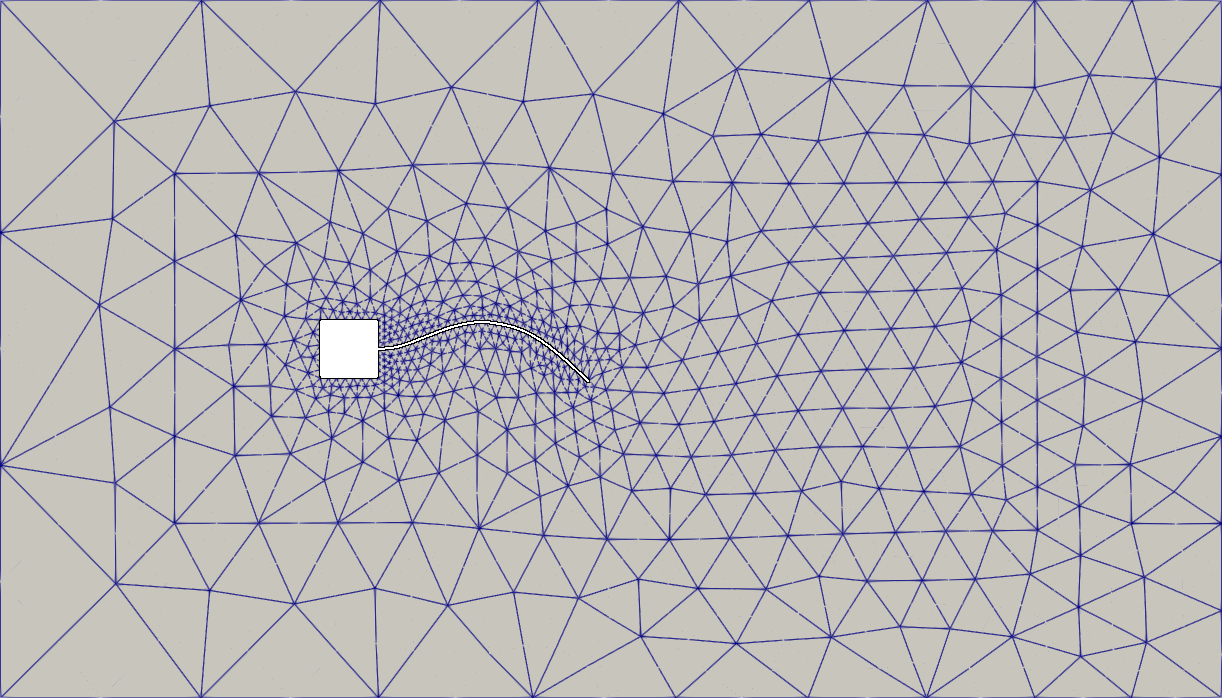
\includegraphics[width=\linewidth]{Figuras/FSI-prism/mT5.png}
        \caption{$t=nT+4T/6$}
    \end{subfigure}
    \begin{subfigure}[b]{0.49\textwidth}
        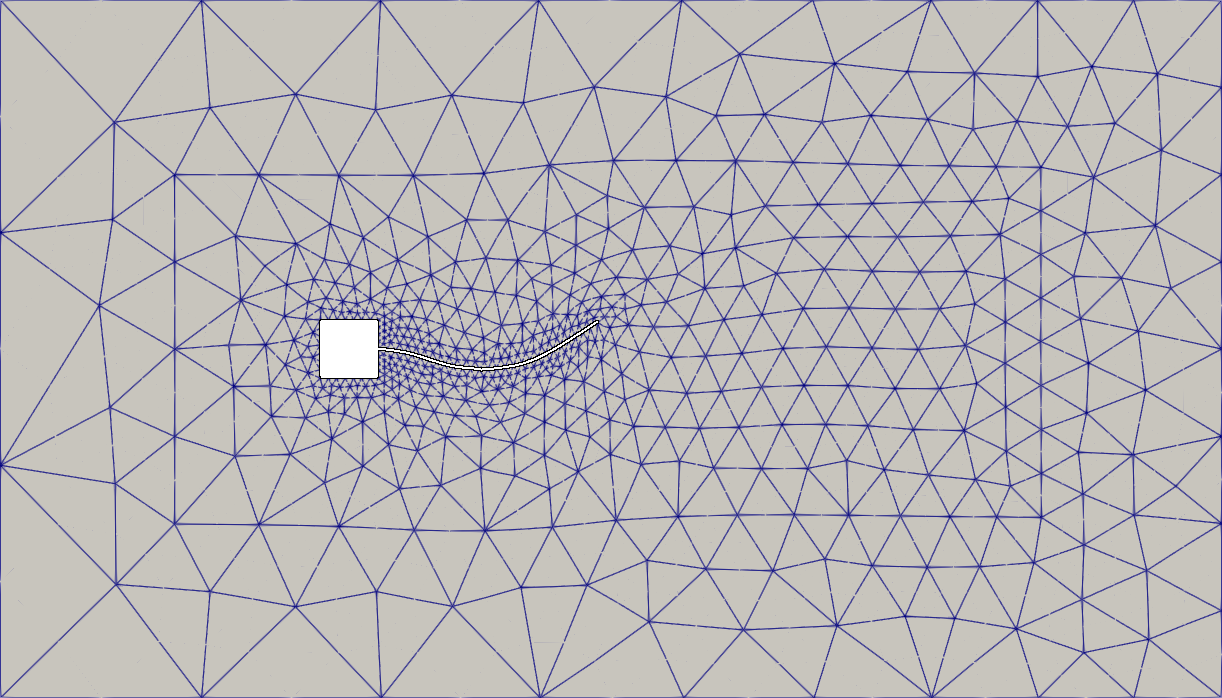
\includegraphics[width=\linewidth]{Figuras/FSI-prism/mT6.png}
        \caption{$t=nT+5T/6$}
    \end{subfigure}
    \\Fonte: Autoria Própria (\the\year).
    \label{fig:prismMesh}
\end{figure}

\textcolor{red}{Quando mudar o exemplo, lembrar de atualizar o coeficiente de Poisson, o raio espectral e a rigidez do elemento}